\chapter{Oscillation Analysis}
\label{chap:OscillationAnalysis}

\section{Likelihood Calculation}
\label{sec:OscillationAnalysis_LLHCalc}

This analysis performs a joint oscillation parameter fit of the ND280,  and the SK atmospheric samples.

Once the Monte Carlo predictions of each beam and atmospheric sample has been built, following from \autoref{chap:SelsAndSysts}, a likelihood needs to be constructed. This is done by comparing the Monte Carlo prediction to ``data''. The data can consist of either an Asmiov Monte Carlo prediction, which is typically used for sensitivity studies, or real data. The Monte Carlo prediction is calculated at a particular point, \quickmath{\vec{\theta}}, in the model parameter space, \quickmath{N_{i}^{MC} = N_{i}^{MC}(\vec{\theta})}. Both the data and Monte Carlo spectra are binned, where the \quickmath{i^{th}} bin content is represented by \quickmath{N_{i}^{D}} and \quickmath{N_{i}^{MC}}, respectively. The bin contents for the beam near detector, beam far detector and atmospheric samples are denoted with \quickmath{ND}, \quickmath{FD} and \quickmath{Atm}, respectively. The binning index, \quickmath{i}, runs over all the bins within the sample and all samples with that set. Taking the beam far detector samples as example, it would run over all the reconstructed neutrino energy bins in all samples (FHC\quickmath{1\text{R}\mu}, RHC\quickmath{1\text{R}\mu}, etc.). The likelihood calculation between data and Monte Carlo for a particular bin follows a Poisson distribution, where the data is treated as a fluctuation of the simulation. 

Following the T2K analysis presented in \cite{Dunne2020-uf}, the likelihood contribution from the near detector also includes a Monte Carlo statistical uncertainty term, derived from the Barlow and Beeston statistical treatment \cite{Barlow1993-cc, Conway2011-go}. In addition to treating the data as a fluctuation of the Monte Carlo prediction, it includes a contribution from the likelihood that the generated simulation is a statistical fluctuation of the actual true simulation assuming infinite statistics. The technical implementation of this additional likelihood term is documented in \cite{t2k_tn_395}. The term is defined as,

\begin{equation}
  \frac{(\beta_{i}-1)^{2}}{2\sigma^{2}_{\beta_{i}}},
\end{equation}

where \quickmath{\beta_{i}} represents a scaling parameter for each bin \quickmath{i}, which is a value based on the amount of Monte Carlo statistics in a bin \cite{t2k_tn_395}. \quickmath{\sigma_{\beta_{i}} = \sqrt{\sum_{i} w_{i}^{2}}/N_{i}^{MC}}, and \quickmath{\sqrt{\sum_{i} w_{i}^{2}}} represents the sum of the square of the weights of the Monte Carlo events which fall into bin \quickmath{i}.

Additional contributions to the likelihood come from the variation of the systematic model parameters. For those parameters with well-motivated uncertainty estimates, a covariance matrix, \quickmath{V} describes the prior knowledge of each parameter as well as any correlations between the parameters. Due to the technical implementation, a single covariance matrix describes each ``block'' of model parameters, e.g. beam flux systematics. For simplicity, the covariance matrix associated with the \quickmath{k^{th}} block is denoted \quickmath{V^{k}}. This substitution results in \quickmath{\vec{\theta} = \sum_{k}^{N_{b}} \vec{\theta}^{k}} and \quickmath{V = \sum_{k}^{N_{b}} V^{k}}, for \quickmath{N_{b}} number of blocks describing: oscillation parameters, beam flux, atmospheric flux, neutrino interaction, near detector, beam far detector and atmospheric far detector systematics detailed in \autoref{sec:SelsAndSysts_Systs}. The number of parameters in the \quickmath{k^{th}} block is defined as \quickmath{n(k)}.

The final likelihood term is defined as,

\begin{align}
\label{eqn:Likelihood:Likelihood}
&-\ln(\mathcal{L}) = \\ 
& \sum_{i}^{\mathsf{ND bins}} N_{i}^{\mathrm{ND},MC}(\vec{\theta}) - N_{i}^{\mathrm{ND},D} + N_{i}^{\mathrm{ND},D}  \times \ln \left[ N_{i}^{\mathrm{ND},D}/N_{i}^{\mathrm{ND},MC}(\vec{\theta}) \right] + \frac{(\beta_{i}-1)^{2}}{2\sigma^{2}_{\beta_{i}}} \nonumber \\
& +  \sum_{i}^{\mathsf{FD bins}} N_{i}^{\mathrm{FD},MC}(\vec{\theta}) - N_{i}^{\mathrm{FD},D} + N_{i}^{\mathrm{FD},D}  \times \ln \left[ N_{i}^{\mathrm{FD},D}/N_{i}^{\mathrm{FD},MC}(\vec{\theta}) \right] \nonumber \\ 
& +  \sum_{i}^{\mathsf{Atm bins}} N_{i}^{\mathrm{Atm},MC}( \vec{\theta}) - N_{i}^{\mathrm{Atm},D} + N_{i}^{\mathrm{Atm},D} \times  \ln \left[ N_{i}^{\mathrm{Atm},D}/N_{i}^{\mathrm{Atm},MC}(\vec{\theta}) \right] \nonumber \\ 
& + \frac{1}{2} \sum_{k}^{N_{b}} \sum_{i}^{n(k)} \sum_{j}^{n(k)} (\vec{\theta}^{k})_{i} (V^{k})^{-1}_{ij} (\vec{\theta}^{k})_{j}. \nonumber
\end{align}

This is the value determined at each step of the MCMC to build the posterior distribution, as discussed in \autoref{chap:MarkovChainMonteCarlo}.

\iffalse
\subsection{Cross-Fitter Validation}
\label{sec:OscillationAnalysis_CrossFitter}

Alongside the analysis presented within this analysis, an alternative fitter \texttt{P-Theta}, has also been developing the analysis. For the purposes of this analysis, the main benefit of the alternative fitter is to validate the response to each parameter. 
\fi

\clearpage
\subsection{Likelihood Scans}
\label{sec:OscillationAnalysis_LLHScans}

Using the defintion of the likelihood presented in \autoref{sec:OscillationAnalysis_LLHCalc}, the response of each sample to a variation particular parameter can be studied. \autoref{fig:OscillationAnalysis_LLHScanOscPars} presents the variation of all the samples (beam and atmospheric) at SK. Each plot represents a ``scan'', where a particular parameter is scanned in some range. The ``data'' being used within the definition of the likelihood equation is built using the Asimov A oscillation parameter values defined in \autoref{tab:Theory_ParameterSets} alongside the pre-fit dial values as discussed in \autoref{sec:SelsAndSysts_Systs_Interaction}. Due to the correlations between oscillation parameters, the value of \quickmath{\chi^{2} \sim 1} does not equate to the typical \quickmath{1\sigma} sensitivity. However, it does give an indication of which samples response the strongest to a variation in the oscillation parameters. The point at which the likelihood tends to zero illustrates the value of the parameter used to build the Asimov data prediction. The likelihood scans only include the sample response and ignore the penalty contribution term from the variation of the parameter.

\begin{figure}[h]
  \begin{subfigure}[t]{0.5\textwidth}
    \includegraphics[width=\textwidth, trim={0mm 0mm 0mm 0mm}, clip,page=4]{Figures/OA/LLHScans_Osc.pdf}
    \subcaption{\quickmath{\sin^{2}(\theta_{23})}}
  \end{subfigure}%
  \begin{subfigure}[t]{0.5\textwidth}
    \includegraphics[width=\textwidth, trim={0mm 0mm 0mm 0mm}, clip,page=7]{Figures/OA/LLHScans_Osc.pdf}
    \subcaption{\quickmath{\Delta m^{2}_{23}}}
  \end{subfigure}
  \begin{subfigure}[t]{0.5\textwidth}
    \includegraphics[width=\textwidth, trim={0mm 0mm 0mm 0mm}, clip,page=8]{Figures/OA/LLHScans_Osc.pdf}
    \subcaption{\quickmath{\delta_{CP}}}
  \end{subfigure}%
  \begin{subfigure}[t]{0.5\textwidth}
    \includegraphics[width=\textwidth, trim={0mm 0mm 0mm 0mm}, clip,page=5]{Figures/OA/LLHScans_Osc.pdf}
    \subcaption{\quickmath{\sin^{2}(\theta_{13})}}
  \end{subfigure}
  \begin{subfigure}[t]{0.5\textwidth}
    \includegraphics[width=\textwidth, trim={0mm 0mm 0mm 0mm}, clip,page=3]{Figures/OA/LLHScans_Osc.pdf}
  \end{subfigure}
  \caption{The response of the likelihood, as defined in \autoref{sec:OscillationAnalysis_LLHCalc}, illustrating the response of the samples to the oscillation parameters. \delmsqsol and \sinsqsol are negated because these samples have no sensitivity to those parameters. The Asimov data set is built using the pre-fit dial values assuming Asimov A oscillation parameters defined in \autoref{tab:Theory_ParameterSets}.}
  \label{fig:OscillationAnalysis_LLHScanOscPars}
\end{figure}

The response to \delmsqatm is much larger in beam samples, specfically \quickmath{\mu}-like samples, compared to atmospheric samples. This is to be expected as the beam neutrino energy can be specifically tuned to match the maximal disappearance probability. As discussed in \autoref{sec:Oscillation_Overview}, the determination of the mass hierarchy is signficantly enhanced when using the atmospheric samples due to them transitioning through the Earth's core. So whilst the atmospheric samples do not add much information to the constraint of \quickmath{|\Delta m^{2}_{32}|} beyond that of the beam analysis, they do enhance the ability to determine the sign of the parameter.

The sensitivity to \sinsqatm is again dominated by the T2K experiment. However, the difference in the response for atmospheric and beam samples is much smaller. Consequently, one would expect that the joint fit would become more sensivity to \sinsqatm than just T2K experiment alone. The summed response over all atmospheric samples becomes comparable to that of the muon-like beam samples. For this particular choice of Asimov point, the only samples which respond to the \sinsqreac parameter are the electron-like beam samples. Consequently, no increase in sensitivity beyond that of the T2K-only analysis is expected at that Asimov point. The \delmsqsol and \sinsqsol are not considered as there is simply no sensitivity in any sample considered within this analysis.
  
As discussed, the correlations between oscillation parameters induce marignalisation effects within the response of the likelihood. That is to say, the response to \dcp is affected by the choice of \sinsqreac or \sinsqatm. The two-dimensional scans of the appearance (\sinsqreac-\dcp) and disappearance (\sinsqatm-\delmsqatm) parameters are illustrated in \autoref{fig:OscillationAnalysis_2DLLHOscScans_App} and \autoref{fig:OscillationAnalysis_2DLLHOscScans_Dis}, respectively.

The appearance log-likelihood scans show the distinct difference in how the beam and atmospheric samples respond. The beam samples have an approximately constant width of the \quickmath{2\sigma} and \quickmath{3\sigma} contours, throughout all ranges of \dcp. The atmospheric samples response to \dcp is very strongly correlated to the choice of \sinsqreac, with the strongest constraints around \quickmath{\delta_{CP}\sim1}. Consequently, this difference allows some of the degeneracy in a beam-only fit to be broken. Comparing the beam and joint fit log-likelihood scans, the \quickmath{2\sigma} continous contour in \dcp for beam samples is broken when the atmospheric samples are added. Furthermore, the width of the \quickmath{3\sigma} contours also becomes dependent upon the value of \dcp. Whilst these are encouraging results for the joint fit, these are not sensitivity measurements as the nuisance parameters are fixed.

The disappearance log-likelihood scans in \sinsqatm-\delmsqatm space show the expected result when considering the one-dimensional scans already discussed. The uncertainty on the width of \quickmath{|\Delta m^{2}_{32}|} is mostly driven by the beam-only sensitivties. However, the width of this contour in the inverted mass region (\quickmath{\Delta m^{2}_{32} < 0}) is significantly reduced due to the ablity of the atmospheric samples to select the correct mass hierarchy (these log-likelihood scans use the Asimov A oscillation probabilities which assumes true normal hierarchy). The width of the uncertainty in \sinsqatm is also reduce compared to a beam-only analysis, with a further decrease in the inverted hierarchy region due to mass hierarchy determination.

\begin{figure}[h]
  \begin{subfigure}[t]{0.5\textwidth}
    \subcaption{Beam Samples}
    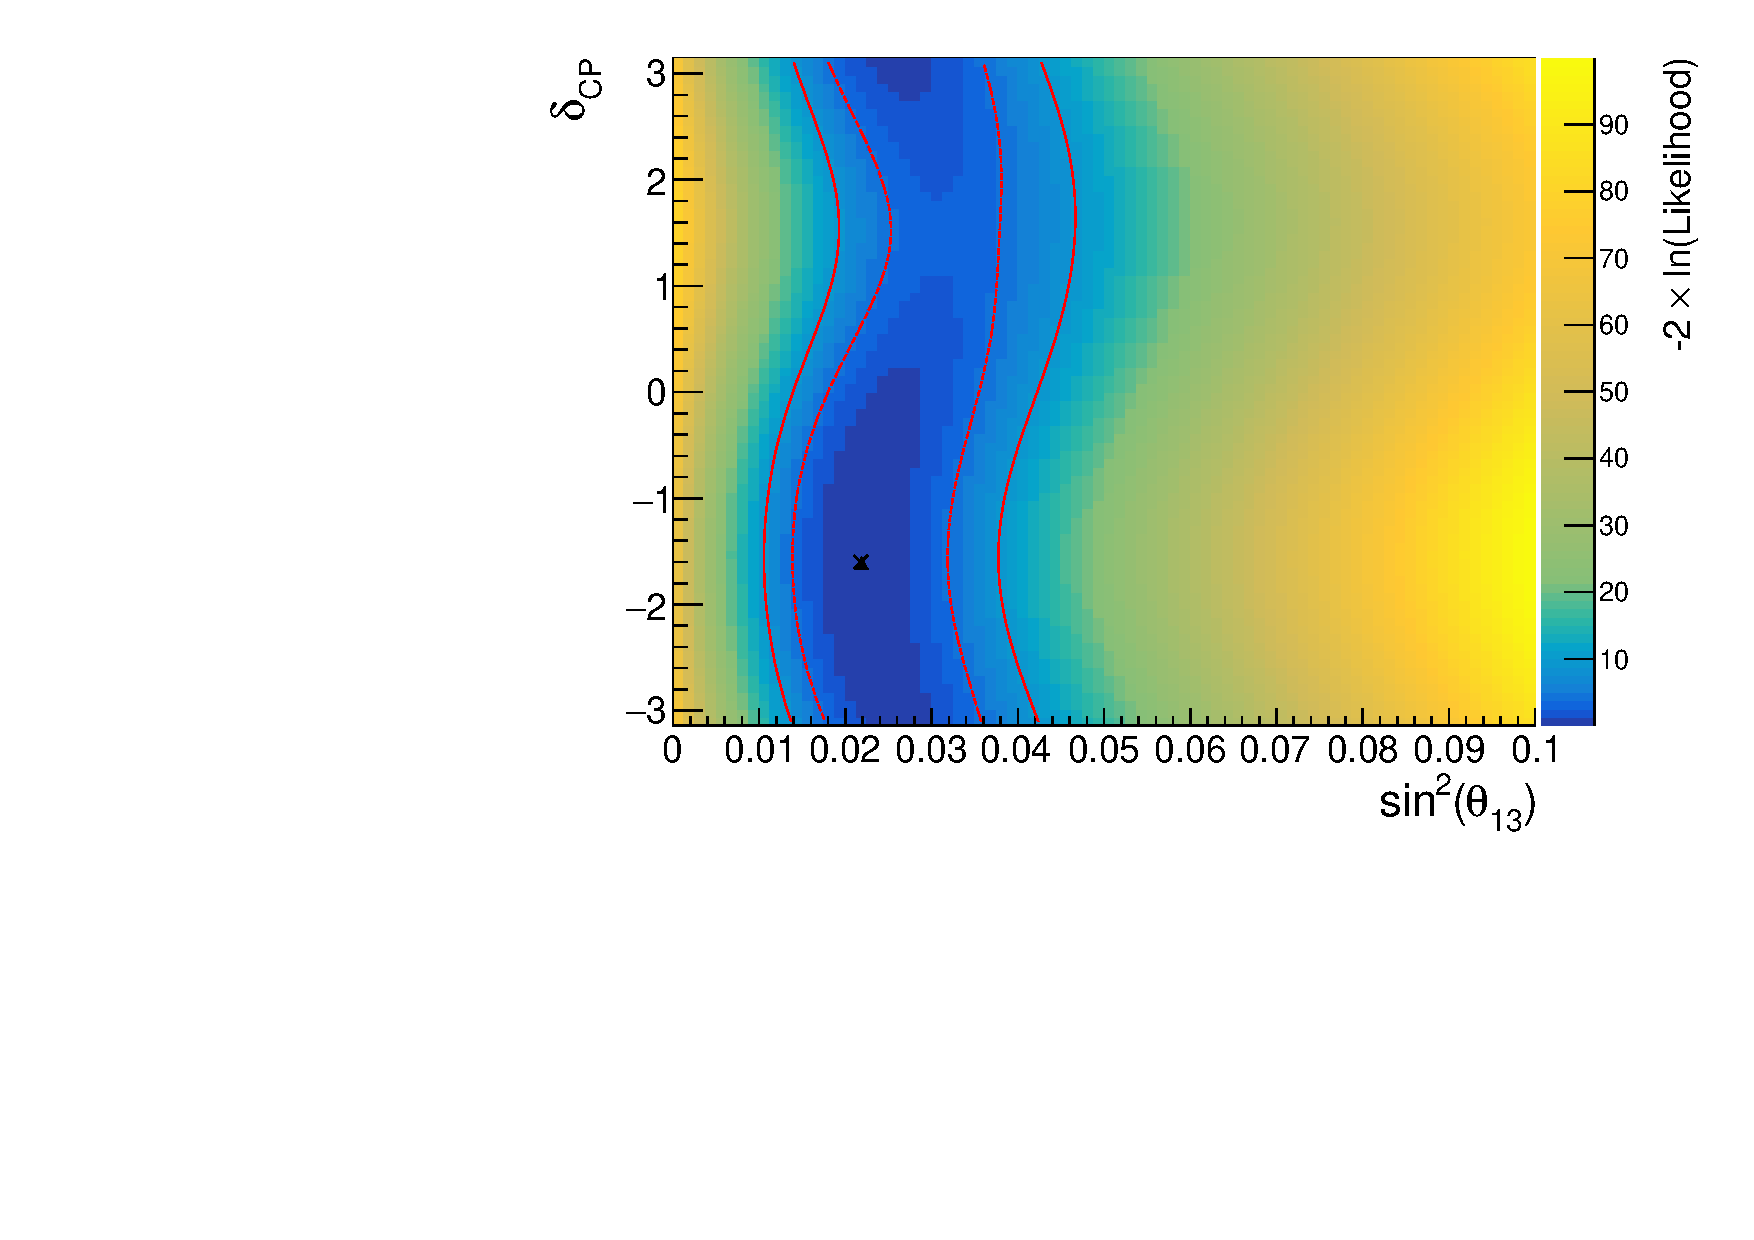
\includegraphics[width=\textwidth, trim={0mm 0mm 0mm 0mm}, clip,page=1]{Figures/OA/AppearanceScans.pdf}
  \end{subfigure}%
  \begin{subfigure}[t]{0.5\textwidth}
    \subcaption{Atmospheric Samples}
    \includegraphics[width=\textwidth, trim={0mm 0mm 0mm 0mm}, clip,page=2]{Figures/OA/AppearanceScans.pdf}
  \end{subfigure}
  \begin{subfigure}[t]{1.0\textwidth}
    \subcaption{All Samples}
    \includegraphics[width=\textwidth, trim={0mm 0mm 0mm 0mm}, clip,page=3]{Figures/OA/AppearanceScans.pdf}
  \end{subfigure}
  \caption{Two-dimensional log-likelihood scan of the appearance (\sinsqreac-\dcp) parameters showing the response of the beam samples (top), atmospheric samples (middle) and the summed response (bottom). The Asimov A oscillation parameters, defined in \autoref{tab:Theory_ParameterSets}, are assumed to be the true point (Black Cross). The position of the smallest log-likelihood is highlighted with the triangle. Prior uncertainty terms of the oscillation parameters are neglected. The two(three) sigma contour levels are illlustrated with the dashed(solid) red line.}
  \label{fig:OscillationAnalysis_2DLLHOscScans_App}
\end{figure}

\begin{figure}[h]
  \begin{subfigure}[t]{0.5\textwidth}
    \subcaption{Beam Samples}
    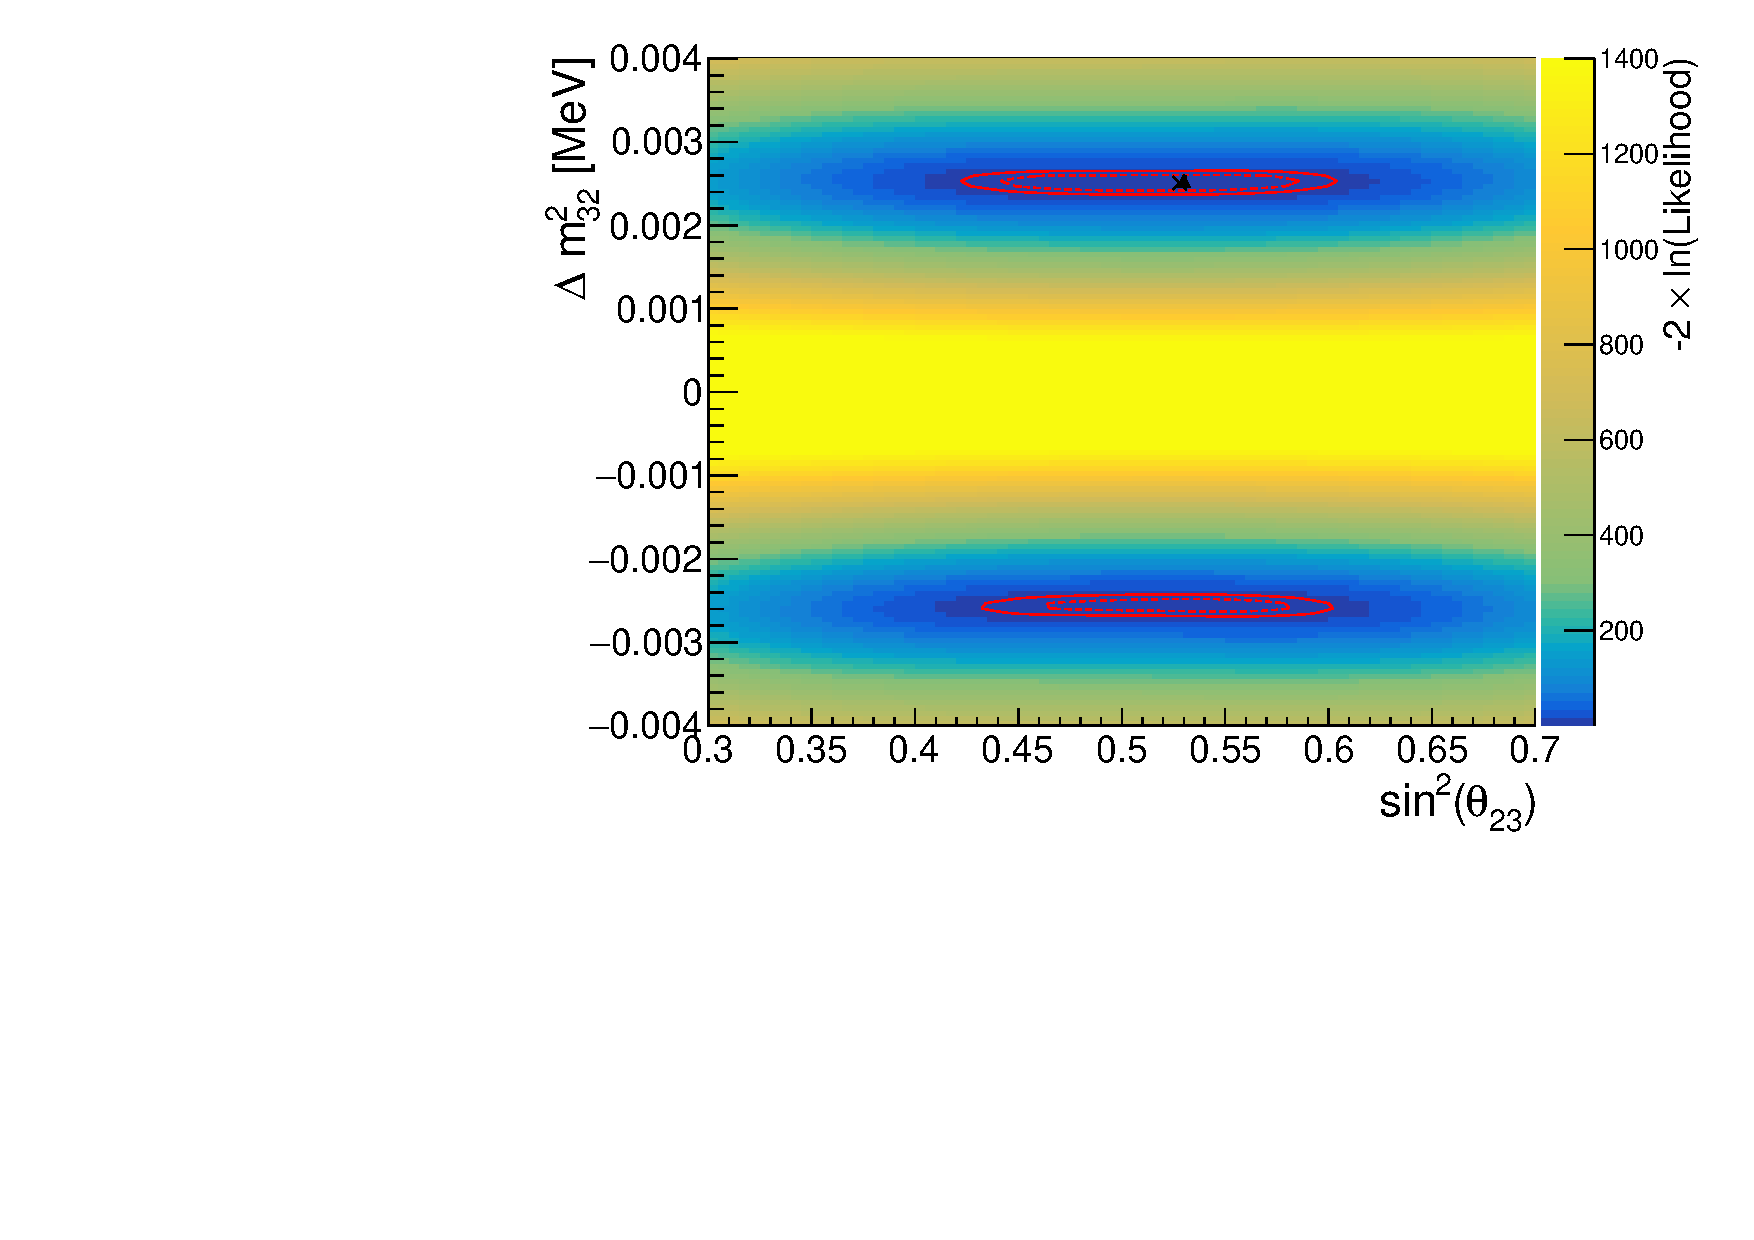
\includegraphics[width=\textwidth, trim={0mm 0mm 0mm 0mm}, clip,page=1]{Figures/OA/DisappearanceScans.pdf}
  \end{subfigure}%
  \begin{subfigure}[t]{0.5\textwidth}
    \subcaption{Atmospheric Samples}
    \includegraphics[width=\textwidth, trim={0mm 0mm 0mm 0mm}, clip,page=2]{Figures/OA/DisappearanceScans.pdf}
  \end{subfigure}
  \begin{subfigure}[t]{1.0\textwidth}
    \subcaption{All Samples}
    \includegraphics[width=\textwidth, trim={0mm 0mm 0mm 0mm}, clip,page=3]{Figures/OA/DisappearanceScans.pdf}
  \end{subfigure}
  \caption{Two-dimensional log-likelihood scan of the disappearance (\sinsqatm-\delmsqatm) parameters showing the response of the beam samples (top), atmospheric samples (middle) and the summed response (bottom). The Asimov A oscillation parameters, defined in \autoref{tab:Theory_ParameterSets}, are assumed to be the true point (Black Cross). The position of the smallest log-likelihood is highlighted with the triangle. Prior uncertainty terms of the oscillation parameters are neglected. The two(three) sigma contour levels are illlustrated with the dashed(solid) red line.}
  \label{fig:OscillationAnalysis_2DLLHOscScans_Dis}
\end{figure}

In addition to the oscillation parameters, the response to the systematic model parameters can also be considered. Due to the correlated cross section model, the most informative \finish{Finish this}

\section{Monte Carlo Prediction}
\label{sec:OscillationAnalysis_MonteCarloPred}

Using the three sets of dial values defined in \autoref{sec:SelsAndSysts_Systs_Interaction}, the predicted event rates for each sample are defined in \autoref{tab:OscillationAnalysis_MCPred}. Both the oscillated event rates assuming Asimov A oscillation parameters (defined in \autoref{tab:Theory_ParameterSets}) and the un-oscillated event rates are given.

\begin{table}[ht!]
    \centering
    \begin{tabular}{|l|c|c|c|c|c|c|}
      \hline
      & \multicolumn{6}{|c|}{Total Predicted Events} \\
      \cline{2-7}
      & \multicolumn{2}{|c}{Generated} & \multicolumn{2}{|c}{Pre-fit} & \multicolumn{2}{|c|}{Post-fit} \\
      \cline{2-7}
      Sample & Osc & UnOsc & Osc & UnOsc & Osc & UnOsc \\
      \hline
      \texttt{SubGeV-elike-0dcy} & 7121.0 & 7102.6 & 6556.8 & 6540.0 & 7035.2 & 7015.7 \\
      \texttt{SubGeV-elike-1dcy} & 704.8 & 725.5 & 693.8 & 712.8 & 565.7 & 586.0 \\
      \texttt{SubGeV-mulike-0dcy} & 1176.5 & 1737.2 & 1078.6 & 1588.1 & 1182.7 & 1757.1 \\
      \texttt{SubGeV-mulike-1dcy} & 5850.7 & 8978.1 & 5351.7 & 8205.1 & 5867.0 & 9009.9 \\
      \texttt{SubGeV-mulike-2dcy} & 446.9 & 655.2 & 441.6 & 647.7 & 345.9 & 505.6 \\
      \texttt{SubGeV-pi0like} & 1438.8 & 1445.4 & 1454.9 & 1461.1 & 1131.1 & 1136.2 \\
      \texttt{MultiGeV-elike-nue} & 201.4 & 195.6 & 201.1 & 195.3 & 202.6 & 196.7 \\
      \texttt{MultiGeV-elike-nuebar} & 1141.5 & 1118.3 & 1060.7 & 1039.5 & 1118.5 & 1095.7 \\
      \texttt{MultiGeV-mulike} & 1036.7 & 1435.8 & 963.1 & 1334.1 & 1015.2 & 1405.9 \\
      \texttt{MultiRing-elike-nue} & 1025.1 & 982.2 & 1026.8 & 984.3 & 1029.8 & 986.4 \\
      \texttt{MultiRing-elike-nuebar} & 1014.8 & 984.5 & 991.0 & 962.0 & 1008.9 & 978.5 \\
      \texttt{MultiRing-mulike} & 2510.0 & 3474.4 & 2475.6 & 3425.8 & 2514.6 & 3480.4 \\      
      \texttt{MultiRingOther-1} & 1204.5 & 1279.1 & 1205.8 & 1280.3 & 1207.4 & 1281.0 \\
      \texttt{PCStop} & 349.2 & 459.2 & 338.4 & 444.7 & 346.8 & 456.1 \\
      \texttt{PCThru} & 1692.8 & 2192.5 & 1661.5 & 2149.8 & 1689.2 & 2187.8 \\
      \texttt{UpStop-mu} & 751.2 & 1295.0 & 739.7 & 1271.6 & 750.4 & 1293.0 \\
      \texttt{UpThruNonShower-mu} & 2584.4 & 3031.6 & 2577.9 & 3019.4 & 2586.8 & 3034.0 \\
      \texttt{UpThruShower-mu} & 473.0 & 488.6 & 473.2 & 488.7 & 473.8 & 489.4 \\
      \texttt{FHC1Rmu} & 328.0 & 1409.2 & 301.1 & 1274.7 & 345.1 & 1568.0 \\
      \texttt{RHC1Rmu} & 133.0 & 432.3 & 122.7 & 396.2 & 135.0 & 443.9 \\
      \texttt{FHC1Re} & 84.6 & 19.2 & 77.4 & 18.2 & 93.7 & 19.7 \\
      \texttt{RHC1Re} & 15.7 & 6.4 & 14.6 & 6.1 & 15.9 & 6.3 \\
      \texttt{FHC1Re1de} & 10.5 & 3.2 & 10.3 & 3.1 & 8.8 & 2.9 \\
      \hline
      \hline
    \end{tabular}
    \caption{The Monte Carlo prediction of each sample observed at SK used within this analysis. Three model parameter tunes are considered, as defined in \autoref{sec:SelsAndSysts_Systs_Interaction}. The oscillated predictions assumed Asimov A oscillation parameters provided in \autoref{tab:Theory_ParameterSets}.}
    \label{tab:OscillationAnalysis_MCPred}
\end{table}

Generally, samples which target CCQE interaction modes observe a decrease in prediction when using the pre-fit dial values. This is in accordance with the Monte Carlo being produced assumed \quickmath{M_{A}^{QE} = 1.21\text{GeV}} whilst the pre-fit dial value should be \quickmath{M_{A}^{QE} = 1.03\text{GeV}}, as suggested by \cite{t2k_tn_344}. Furthermore, the predicted event rates of samples which target CCRES interaction modes is significantly reduced when considering the post-ND fit. This follows the observations in \autoref{sec:SelsAndSysts_Systs_Interaction}. The strength of the accelerator neutrino experiment can also be seen in the remarkable difference between the oscillated and unoscillated predictions in the \texttt{FHC1Rmu} and \texttt{RHC1Rmu} samples. There is a very obvious decrease in the expected event rate between the two predictions which is not as clearly observed in the atmospheric samples. This is due to the fact that the beam energy is tuned to the maximum disappearance probability, which is not the case for the naturally generated atmospheric neutrinos.

